% Options for packages loaded elsewhere
\PassOptionsToPackage{unicode}{hyperref}
\PassOptionsToPackage{hyphens}{url}
%
\documentclass[
]{article}
\usepackage{amsmath,amssymb}
\usepackage{lmodern}
\usepackage{ifxetex,ifluatex}
\ifnum 0\ifxetex 1\fi\ifluatex 1\fi=0 % if pdftex
  \usepackage[T1]{fontenc}
  \usepackage[utf8]{inputenc}
  \usepackage{textcomp} % provide euro and other symbols
\else % if luatex or xetex
  \usepackage{unicode-math}
  \defaultfontfeatures{Scale=MatchLowercase}
  \defaultfontfeatures[\rmfamily]{Ligatures=TeX,Scale=1}
\fi
% Use upquote if available, for straight quotes in verbatim environments
\IfFileExists{upquote.sty}{\usepackage{upquote}}{}
\IfFileExists{microtype.sty}{% use microtype if available
  \usepackage[]{microtype}
  \UseMicrotypeSet[protrusion]{basicmath} % disable protrusion for tt fonts
}{}
\makeatletter
\@ifundefined{KOMAClassName}{% if non-KOMA class
  \IfFileExists{parskip.sty}{%
    \usepackage{parskip}
  }{% else
    \setlength{\parindent}{0pt}
    \setlength{\parskip}{6pt plus 2pt minus 1pt}}
}{% if KOMA class
  \KOMAoptions{parskip=half}}
\makeatother
\usepackage{xcolor}
\IfFileExists{xurl.sty}{\usepackage{xurl}}{} % add URL line breaks if available
\IfFileExists{bookmark.sty}{\usepackage{bookmark}}{\usepackage{hyperref}}
\hypersetup{
  pdftitle={Bike Lanes \& Gentrification in Los Angeles},
  pdfauthor={E.Sheild\_N.Levine\_G.Barrett-Jackson},
  hidelinks,
  pdfcreator={LaTeX via pandoc}}
\urlstyle{same} % disable monospaced font for URLs
\usepackage[margin=1in]{geometry}
\usepackage{longtable,booktabs,array}
\usepackage{calc} % for calculating minipage widths
% Correct order of tables after \paragraph or \subparagraph
\usepackage{etoolbox}
\makeatletter
\patchcmd\longtable{\par}{\if@noskipsec\mbox{}\fi\par}{}{}
\makeatother
% Allow footnotes in longtable head/foot
\IfFileExists{footnotehyper.sty}{\usepackage{footnotehyper}}{\usepackage{footnote}}
\makesavenoteenv{longtable}
\usepackage{graphicx}
\makeatletter
\def\maxwidth{\ifdim\Gin@nat@width>\linewidth\linewidth\else\Gin@nat@width\fi}
\def\maxheight{\ifdim\Gin@nat@height>\textheight\textheight\else\Gin@nat@height\fi}
\makeatother
% Scale images if necessary, so that they will not overflow the page
% margins by default, and it is still possible to overwrite the defaults
% using explicit options in \includegraphics[width, height, ...]{}
\setkeys{Gin}{width=\maxwidth,height=\maxheight,keepaspectratio}
% Set default figure placement to htbp
\makeatletter
\def\fps@figure{htbp}
\makeatother
\setlength{\emergencystretch}{3em} % prevent overfull lines
\providecommand{\tightlist}{%
  \setlength{\itemsep}{0pt}\setlength{\parskip}{0pt}}
\setcounter{secnumdepth}{-\maxdimen} % remove section numbering
\usepackage{array}
\usepackage{caption}
\usepackage{graphicx}
\usepackage{siunitx}
\usepackage[normalem]{ulem}
\usepackage{colortbl}
\usepackage{multirow}
\usepackage{hhline}
\usepackage{calc}
\usepackage{tabularx}
\usepackage{threeparttable}
\usepackage{wrapfig}
\usepackage{adjustbox}
\usepackage{hyperref}
\ifluatex
  \usepackage{selnolig}  % disable illegal ligatures
\fi

\title{Bike Lanes \& Gentrification in Los Angeles}
\author{E.Sheild\_N.Levine\_G.Barrett-Jackson}
\date{12/1/21}

\begin{document}
\maketitle

{
\setcounter{tocdepth}{3}
\tableofcontents
}
{[}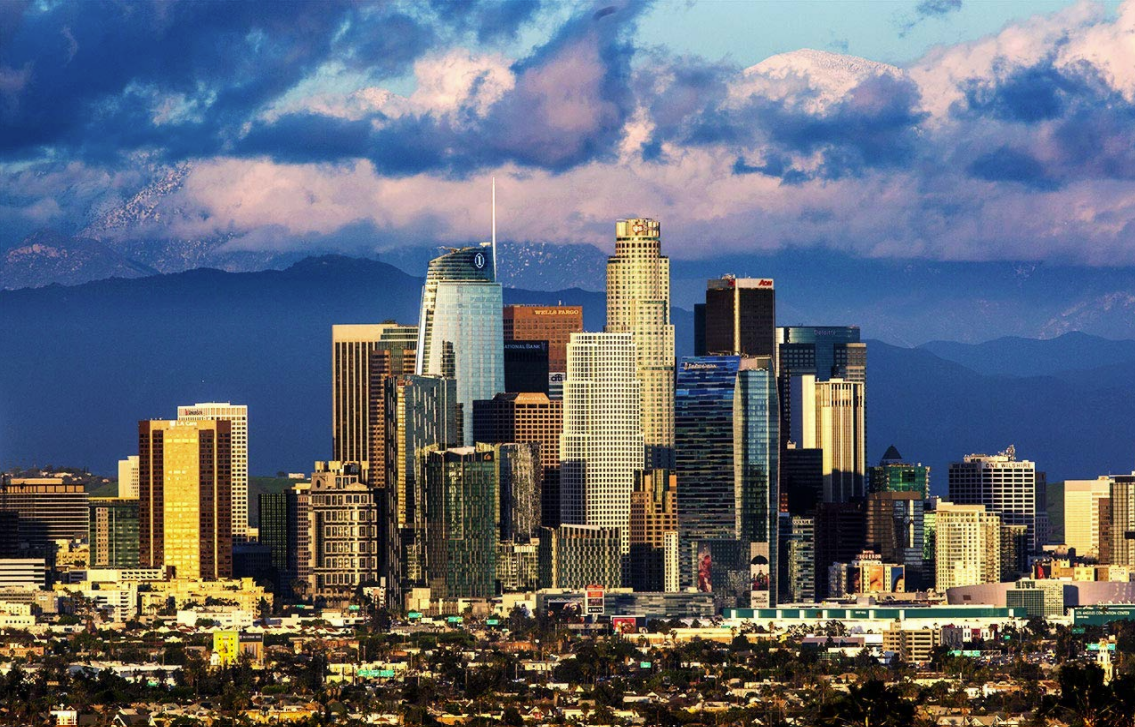
\includegraphics{Quant-main/thumbnails/LA.png}{]}

Above image courtesy of TravLin Photography. \# Introduction

Noting environmental, health, and other benefits, more and more
municipalities are implementing complete streets plans that emphasize
sustainable modes of transportation like biking. Advocates of these
plans present them as a panacea for pollution, air quality, and
congestion, among other ills. Challenging this rosy narrative, however,
critics have posited a link between bicycle infrastructure and
gentrification, citing anecdotal evidence of displacement in the wake of
its installation.

This semester, we set out to test this empirically. With respect to the
City of Los Angeles, we ask, what is the relationship between the
installation of bicycle infrastructure and gentrification? On the basis
of our lived experience in the region, we hypothesize that there is a
positive relationship between the installation of bicycle infrastructure
and gentrification.

\hypertarget{background}{%
\section{Background}\label{background}}

In order to understand the socioeconomic implications of bicycle
infrastructure, we first contextualize previous academic research
supplemented with current news articles.

Exploring the relationship between the installation of bicycle
facilities and socioeconomic and demographic changes in 29 US cities,
Ferenchak and Wesley researched the distribution of bicycling networks
across socioeconomic/demographic spectrums (2021). Their research
concluded that while bike lane installation was concentrated in
lower-income areas, there was a ``weak and largely non-significant''
relationship of causality.

Focusing on Portland, OR and Chicago, IL, Flanagan et al.~(2016)
``identify a bias towards increased cycling infrastructure investment in
areas of existing or increasing privilege.'' Reviewing research methods
used in this study was an important roadmap for us as the researchers
pulled from census demographic data and ran linear regressions to
estimate how changes in demographics associated with gentrification are
related to cycling infrastructure investment.

Finally, we relied heavily on the teachings and research of our
Professor, Carole Voulgaris. Her publication with other researches
``Healthy for whom? Equity in the spatial distribution of cycling risks
in Los Angeles, CA'' provided good research methodological strategy and
structure as well as inspired us to keep equity at the forefront of our
research (Braun et. al., 2021).

Ahead of diving into our own data in the context of Los Angeles, these
research bodies, and current news articles, helped us to think
critically about our research question and hypothesis. We hope our
research can supplement and contribute to the broader research body of
social determinants of bicycle infrastructure and ridership.

\hypertarget{data}{%
\section{Data}\label{data}}

We have conceptualized bicycle infrastructure in terms of means of
transportation to work and bike lane length. We have conceptualized
gentrification in terms of tenure, race, and median income.

The sample population for this study is the all census tracts in the
City of Los Angeles. The analysis included the following categorical and
continuous variables:

\begin{itemize}
\tightlist
\item
  Tenure: 2019 American Communities Survey, ``Did this person live in
  this house or apartment 5 years ago?''
\item
  Race (White): 2019 American Communities Survey, ``What is Person 1's
  race?''
\item
  Median Income (\$): 2019 American Communities Survey, ``What was this
  person's total income during the past 12 months?''
\item
  Means of Transportation (Bike): 2019 American Communities Survey,
  ``How did this person usually get to work last week?''
\item
  Bikeways (Linear Feet): LACity GeoHub. This is our selected dependent
  variable that depends on and is influenced by all the other
  independent variables.
\end{itemize}

We pulled data from the American Communities Survey (ACS). To define
bicycle infrastructure we settled on the amount of bike lane length
(linear feet) per census tract. To accomplish this we retrieved a
shapefile containing all the bike lanes in the City of LA through LA
City GeoHub, uploaded that shapefile to ArcGIS Pro, clipped the bike
lanes to a LA City census tract shapefile, used ArcGIS Pro's ``summarize
within'' function to calculate the bike lane length (linear feet) per
census tract.

To narrow our scope and further define bike infrastructure, we only
included Lane (69.98\%), Protected Bike Lane (2.38\%), Buffer Bike Lane
(1.08\%), and Path (0.75\%), and excluded Sharrowed Route (14.48\%),
Route (11.04\%), Bicycle Friendly Street (0.17\%), Temp Removal
Sharrowed Route (0.08\%), and Detour Sharrowed Route (0.03\%).

\includegraphics{index_files/figure-latex/unnamed-chunk-18-1.pdf}
\includegraphics{index_files/figure-latex/unnamed-chunk-18-2.pdf}
\includegraphics{index_files/figure-latex/unnamed-chunk-18-3.pdf}
\includegraphics{index_files/figure-latex/unnamed-chunk-18-4.pdf}

\hypertarget{descriptive-statistics}{%
\subsection{Descriptive Statistics}\label{descriptive-statistics}}

The below descriptive statistics table provides an overview of our data.

\begin{longtable}[]{@{}
  >{\raggedright\arraybackslash}p{(\columnwidth - 12\tabcolsep) * \real{0.12}}
  >{\raggedleft\arraybackslash}p{(\columnwidth - 12\tabcolsep) * \real{0.08}}
  >{\raggedleft\arraybackslash}p{(\columnwidth - 12\tabcolsep) * \real{0.25}}
  >{\raggedleft\arraybackslash}p{(\columnwidth - 12\tabcolsep) * \real{0.25}}
  >{\raggedleft\arraybackslash}p{(\columnwidth - 12\tabcolsep) * \real{0.05}}
  >{\raggedleft\arraybackslash}p{(\columnwidth - 12\tabcolsep) * \real{0.13}}
  >{\raggedleft\arraybackslash}p{(\columnwidth - 12\tabcolsep) * \real{0.12}}@{}}
\toprule
Variable & Sample mean & Population mean (95\% confidence) - low &
Population mean (95\% confidence) - high & Median & Interquartile range
& Standard deviation \\
\midrule
\endhead
Median Income (\$) & 33279 & 32222 & 34335 & 26518 & 20642 & 16967 \\
Transport (People) & 19 & 17 & 21 & 8 & 25 & 32 \\
Median Age (Years) & 36 & 36 & 37 & 36 & 8 & 6 \\
Bikeways (Feet) & 3262788 & 2914187 & 3611389 & 1970129 & 4069 &
5295887 \\
\bottomrule
\end{longtable}

\hypertarget{formatted-table-for-white-population}{%
\subsubsection{Formatted table for white
population}\label{formatted-table-for-white-population}}

\hypertarget{formatted-table-for-tenure}{%
\subsubsection{Formatted table for
Tenure}\label{formatted-table-for-tenure}}

\begin{longtable}[]{@{}
  >{\raggedright\arraybackslash}p{(\columnwidth - 6\tabcolsep) * \real{0.24}}
  >{\raggedleft\arraybackslash}p{(\columnwidth - 6\tabcolsep) * \real{0.18}}
  >{\raggedleft\arraybackslash}p{(\columnwidth - 6\tabcolsep) * \real{0.28}}
  >{\raggedleft\arraybackslash}p{(\columnwidth - 6\tabcolsep) * \real{0.29}}@{}}
\toprule
Tenure in Census Tracts & Sample proportion & 95-percent confidence -
low & 95-percent confidence - high \\
\midrule
\endhead
New Residents & 0.9888507 & 0.8777612 & 1.09994 \\
\bottomrule
\end{longtable}

\hypertarget{bar-chart-white}{%
\subsubsection{Bar Chart \% white}\label{bar-chart-white}}

\includegraphics{index_files/figure-latex/unnamed-chunk-24-1.pdf}

\hypertarget{methods}{%
\section{Methods}\label{methods}}

After conducting our previous research and collecting our datasets, our
research methods consisted of organizing, filtering, and compiling our
data set and then ran a series linear regressions to analyze the linear
of feet of bike lanes to the gentrification variables. Linear feet of
bike lane per census tract was our dependent variable. Although
interpreted in greater detail in the previous section, the purpose of
this study is to assess whether bike lane length per census tracts is an
indicator of areas of greater gentrification. Therefore, if our model
has a significant positive coefficient for majority white, that means
majority white census tracts have more bicycle lanes.

The first linear regression is a bi-variate analysis. A bi-variate
relationship is between two variables, race (white) and bikeways
(dependent). Put simply, a regression, which is all about prediction on
an average, is a method for determining the relationship between
quantifiable variables.

Secondly, we ran a series of multivariate regressions to control for the
other independent variables. This regression model, lm function,
predicts the effects of the change in gentrification on the linear feet
of bike lanes.

Thirdly, based on our variables, we believe the non-linear
transformation is a better fit for our data. We want to analyze if the
\% change in our variables is a better indicator than the actual value
of a fixed increase/decrease. This statistical significance of
pop\_density to bike lane length inspired us to run log2, which with a
base-two log our interpretation of the coefficient will have the effect
of doubling the population density.

Lastly, based on the results of our log transformation we have decided
to interact median income with majority white and majority non-white
census tracts. An interaction is like a test to see the relationship
between one of your dependent variables, bike lane length, and
independent variable, median income. We are curious if the relationship
between median income and bike lane length depends on the majority race
in a tract. In the below section are the results and interpretations of
each.

\hypertarget{bivariate-analysis}{%
\subsection{Bivariate Analysis}\label{bivariate-analysis}}

\hypertarget{median-income}{%
\subsubsection{Median Income}\label{median-income}}

In running a bivariate analysis between these two continuous variables,
our 95\% confidence interval does not include zero, and all values are
positive. The correlation coefficient leads us to conclude, with 95\%
confidence, that there is a weak positive relationship between length of
bike lanes and median income per census tract.

\hypertarget{binary-white}{%
\subsubsection{Binary White}\label{binary-white}}

In our bivariate regression with binary\_whitewhite (white majority
census tracts) and sum\_Length (feet of bike lane per census tract), we
found, on average, that white majority census tracts in Los Angeles have
794.1 more feet of bike lane than non-white majority census tracts. This
finding was significant at the 99\% confidence level.

\hypertarget{population-density}{%
\subsubsection{Population Density}\label{population-density}}

Since the confidence interval includes zero, we cannot say with 95\%
certainty that bikeway length is associated with population density,
however we still find this to be helpful to our research in
acknowledging that bike lane length amount neither has a strong negative
or positive correlation (with 95\% certainty) with population density.

\hypertarget{multivariate-analysis}{%
\subsection{Multivariate Analysis}\label{multivariate-analysis}}

 
  \providecommand{\huxb}[2]{\arrayrulecolor[RGB]{#1}\global\arrayrulewidth=#2pt}
  \providecommand{\huxvb}[2]{\color[RGB]{#1}\vrule width #2pt}
  \providecommand{\huxtpad}[1]{\rule{0pt}{#1}}
  \providecommand{\huxbpad}[1]{\rule[-#1]{0pt}{#1}}

\begin{table}[ht]
\begin{centerbox}
\begin{threeparttable}
 \label{tab:unnamed-chunk-36}
\setlength{\tabcolsep}{0pt}
\begin{tabular}{l l l}


\hhline{>{\huxb{0, 0, 0}{0.8}}->{\huxb{0, 0, 0}{0.8}}->{\huxb{0, 0, 0}{0.8}}-}
\arrayrulecolor{black}

\multicolumn{1}{!{\huxvb{0, 0, 0}{0}}c!{\huxvb{0, 0, 0}{0}}}{\huxtpad{6pt + 1em}\centering \hspace{6pt}  \hspace{6pt}\huxbpad{6pt}} &
\multicolumn{1}{c!{\huxvb{0, 0, 0}{0}}}{\huxtpad{6pt + 1em}\centering \hspace{6pt} Initial \hspace{6pt}\huxbpad{6pt}} &
\multicolumn{1}{c!{\huxvb{0, 0, 0}{0}}}{\huxtpad{6pt + 1em}\centering \hspace{6pt} Logged \hspace{6pt}\huxbpad{6pt}} \tabularnewline[-0.5pt]


\hhline{>{\huxb{255, 255, 255}{0.4}}->{\huxb{0, 0, 0}{0.4}}->{\huxb{0, 0, 0}{0.4}}-}
\arrayrulecolor{black}

\multicolumn{1}{!{\huxvb{0, 0, 0}{0}}l!{\huxvb{0, 0, 0}{0}}}{\huxtpad{6pt + 1em}\raggedright \hspace{6pt} Constant \hspace{6pt}\huxbpad{6pt}} &
\multicolumn{1}{r!{\huxvb{0, 0, 0}{0}}}{\huxtpad{6pt + 1em}\raggedleft \hspace{6pt} 4662.96 *** (p = 0.00) \hspace{6pt}\huxbpad{6pt}} &
\multicolumn{1}{r!{\huxvb{0, 0, 0}{0}}}{\huxtpad{6pt + 1em}\raggedleft \hspace{6pt} 24642.75 *** (p = 0.00) \hspace{6pt}\huxbpad{6pt}} \tabularnewline[-0.5pt]


\hhline{}
\arrayrulecolor{black}

\multicolumn{1}{!{\huxvb{0, 0, 0}{0}}l!{\huxvb{0, 0, 0}{0}}}{\huxtpad{6pt + 1em}\raggedright \hspace{6pt} New residents (\%) \hspace{6pt}\huxbpad{6pt}} &
\multicolumn{1}{r!{\huxvb{0, 0, 0}{0}}}{\huxtpad{6pt + 1em}\raggedleft \hspace{6pt} 15206.92 (p = 0.06) \hspace{6pt}\huxbpad{6pt}} &
\multicolumn{1}{r!{\huxvb{0, 0, 0}{0}}}{\huxtpad{6pt + 1em}\raggedleft \hspace{6pt} 14521.55 (p = 0.06) \hspace{6pt}\huxbpad{6pt}} \tabularnewline[-0.5pt]


\hhline{}
\arrayrulecolor{black}

\multicolumn{1}{!{\huxvb{0, 0, 0}{0}}l!{\huxvb{0, 0, 0}{0}}}{\huxtpad{6pt + 1em}\raggedright \hspace{6pt} Majority white (binary) \hspace{6pt}\huxbpad{6pt}} &
\multicolumn{1}{r!{\huxvb{0, 0, 0}{0}}}{\huxtpad{6pt + 1em}\raggedleft \hspace{6pt} 153.62 (p = 0.63) \hspace{6pt}\huxbpad{6pt}} &
\multicolumn{1}{r!{\huxvb{0, 0, 0}{0}}}{\huxtpad{6pt + 1em}\raggedleft \hspace{6pt} 14.67 (p = 0.96) \hspace{6pt}\huxbpad{6pt}} \tabularnewline[-0.5pt]


\hhline{}
\arrayrulecolor{black}

\multicolumn{1}{!{\huxvb{0, 0, 0}{0}}l!{\huxvb{0, 0, 0}{0}}}{\huxtpad{6pt + 1em}\raggedright \hspace{6pt} Log population density (people/sqmi) \hspace{6pt}\huxbpad{6pt}} &
\multicolumn{1}{r!{\huxvb{0, 0, 0}{0}}}{\huxtpad{6pt + 1em}\raggedleft \hspace{6pt}  \hphantom{0}\hphantom{0}\hphantom{0}\hphantom{0} \hspace{6pt}\huxbpad{6pt}} &
\multicolumn{1}{r!{\huxvb{0, 0, 0}{0}}}{\huxtpad{6pt + 1em}\raggedleft \hspace{6pt} -2169.78 *** (p = 0.00) \hspace{6pt}\huxbpad{6pt}} \tabularnewline[-0.5pt]


\hhline{}
\arrayrulecolor{black}

\multicolumn{1}{!{\huxvb{0, 0, 0}{0}}l!{\huxvb{0, 0, 0}{0}}}{\huxtpad{6pt + 1em}\raggedright \hspace{6pt} Median income (\$) \hspace{6pt}\huxbpad{6pt}} &
\multicolumn{1}{r!{\huxvb{0, 0, 0}{0}}}{\huxtpad{6pt + 1em}\raggedleft \hspace{6pt} -0.01 (p = 0.37) \hspace{6pt}\huxbpad{6pt}} &
\multicolumn{1}{r!{\huxvb{0, 0, 0}{0}}}{\huxtpad{6pt + 1em}\raggedleft \hspace{6pt} -0.04 *** (p = 0.00) \hspace{6pt}\huxbpad{6pt}} \tabularnewline[-0.5pt]


\hhline{}
\arrayrulecolor{black}

\multicolumn{1}{!{\huxvb{0, 0, 0}{0}}l!{\huxvb{0, 0, 0}{0}}}{\huxtpad{6pt + 1em}\raggedright \hspace{6pt} Bike commuters (\%) \hspace{6pt}\huxbpad{6pt}} &
\multicolumn{1}{r!{\huxvb{0, 0, 0}{0}}}{\huxtpad{6pt + 1em}\raggedleft \hspace{6pt} 4912.19 (p = 0.78) \hspace{6pt}\huxbpad{6pt}} &
\multicolumn{1}{r!{\huxvb{0, 0, 0}{0}}}{\huxtpad{6pt + 1em}\raggedleft \hspace{6pt} 26057.00 (p = 0.12) \hspace{6pt}\huxbpad{6pt}} \tabularnewline[-0.5pt]


\hhline{>{\huxb{255, 255, 255}{0.4}}->{\huxb{0, 0, 0}{0.4}}->{\huxb{0, 0, 0}{0.4}}-}
\arrayrulecolor{black}

\multicolumn{1}{!{\huxvb{0, 0, 0}{0}}l!{\huxvb{0, 0, 0}{0}}}{\huxtpad{6pt + 1em}\raggedright \hspace{6pt} N \hspace{6pt}\huxbpad{6pt}} &
\multicolumn{1}{r!{\huxvb{0, 0, 0}{0}}}{\huxtpad{6pt + 1em}\raggedleft \hspace{6pt} 881\hphantom{0}\hphantom{0}\hphantom{0}\hphantom{0} \hspace{6pt}\huxbpad{6pt}} &
\multicolumn{1}{r!{\huxvb{0, 0, 0}{0}}}{\huxtpad{6pt + 1em}\raggedleft \hspace{6pt} 881\hphantom{0}\hphantom{0}\hphantom{0}\hphantom{0} \hspace{6pt}\huxbpad{6pt}} \tabularnewline[-0.5pt]


\hhline{}
\arrayrulecolor{black}

\multicolumn{1}{!{\huxvb{0, 0, 0}{0}}l!{\huxvb{0, 0, 0}{0}}}{\huxtpad{6pt + 1em}\raggedright \hspace{6pt} R2 \hspace{6pt}\huxbpad{6pt}} &
\multicolumn{1}{r!{\huxvb{0, 0, 0}{0}}}{\huxtpad{6pt + 1em}\raggedleft \hspace{6pt} 0.09\hphantom{0} \hspace{6pt}\huxbpad{6pt}} &
\multicolumn{1}{r!{\huxvb{0, 0, 0}{0}}}{\huxtpad{6pt + 1em}\raggedleft \hspace{6pt} 0.18\hphantom{0} \hspace{6pt}\huxbpad{6pt}} \tabularnewline[-0.5pt]


\hhline{>{\huxb{0, 0, 0}{0.8}}->{\huxb{0, 0, 0}{0.8}}->{\huxb{0, 0, 0}{0.8}}-}
\arrayrulecolor{black}

\multicolumn{3}{!{\huxvb{0, 0, 0}{0}}l!{\huxvb{0, 0, 0}{0}}}{\huxtpad{6pt + 1em}\raggedright \hspace{6pt}  *** p $<$ 0.001;  ** p $<$ 0.01;  * p $<$ 0.05. \hspace{6pt}\huxbpad{6pt}} \tabularnewline[-0.5pt]


\hhline{}
\arrayrulecolor{black}
\end{tabular}
\end{threeparttable}\par\end{centerbox}

\end{table}
 

For our multivariate analysis (Initial), which yielded a statistically
significant negative correlation of pop density and bike lane length.
For every additional linear foot of bike lane, the average census tract
``loses'' .09 people per square mile. The R-squared explains 9\% of the
variation in sum length while our old R-squared (full\_model, without
the new variables) explains 2.1\% of the variation in sum length, so our
new model is a better fit. After we log transformed population density
and re-ran the regression, log\_pop\_density retained its significance
and med\_income\_E also became statistically significant. The R-squared
value tells how much of the variation in the dependent variable is due
to the other independent variables. Our R-squared is .1779 for the log
transformation, which is up from .086. This means that our model now
explains 17.79\% of the variation in the dependent variable (rounded to
18\% in the cleaner table).\\
Overall, we argue that the non-linear transformation, using a base-two
log, is in fact a better predictor of change and does make our data
easier to interpret.

\hypertarget{interactions}{%
\subsection{Interactions}\label{interactions}}

 
  \providecommand{\huxb}[2]{\arrayrulecolor[RGB]{#1}\global\arrayrulewidth=#2pt}
  \providecommand{\huxvb}[2]{\color[RGB]{#1}\vrule width #2pt}
  \providecommand{\huxtpad}[1]{\rule{0pt}{#1}}
  \providecommand{\huxbpad}[1]{\rule[-#1]{0pt}{#1}}

\begin{table}[ht]
\begin{centerbox}
\begin{threeparttable}
 \label{tab:unnamed-chunk-37}
\setlength{\tabcolsep}{0pt}
\begin{tabular}{l l l}


\hhline{>{\huxb{0, 0, 0}{0.8}}->{\huxb{0, 0, 0}{0.8}}->{\huxb{0, 0, 0}{0.8}}-}
\arrayrulecolor{black}

\multicolumn{1}{!{\huxvb{0, 0, 0}{0}}c!{\huxvb{0, 0, 0}{0}}}{\huxtpad{6pt + 1em}\centering \hspace{6pt}  \hspace{6pt}\huxbpad{6pt}} &
\multicolumn{1}{c!{\huxvb{0, 0, 0}{0}}}{\huxtpad{6pt + 1em}\centering \hspace{6pt} Logged \hspace{6pt}\huxbpad{6pt}} &
\multicolumn{1}{c!{\huxvb{0, 0, 0}{0}}}{\huxtpad{6pt + 1em}\centering \hspace{6pt} Interaction \hspace{6pt}\huxbpad{6pt}} \tabularnewline[-0.5pt]


\hhline{>{\huxb{255, 255, 255}{0.4}}->{\huxb{0, 0, 0}{0.4}}->{\huxb{0, 0, 0}{0.4}}-}
\arrayrulecolor{black}

\multicolumn{1}{!{\huxvb{0, 0, 0}{0}}l!{\huxvb{0, 0, 0}{0}}}{\huxtpad{6pt + 1em}\raggedright \hspace{6pt} (Intercept) \hspace{6pt}\huxbpad{6pt}} &
\multicolumn{1}{r!{\huxvb{0, 0, 0}{0}}}{\huxtpad{6pt + 1em}\raggedleft \hspace{6pt} 24642.75 *** (p = 0.00) \hspace{6pt}\huxbpad{6pt}} &
\multicolumn{1}{r!{\huxvb{0, 0, 0}{0}}}{\huxtpad{6pt + 1em}\raggedleft \hspace{6pt} 22432.30 *** (p = 0.00) \hspace{6pt}\huxbpad{6pt}} \tabularnewline[-0.5pt]


\hhline{}
\arrayrulecolor{black}

\multicolumn{1}{!{\huxvb{0, 0, 0}{0}}l!{\huxvb{0, 0, 0}{0}}}{\huxtpad{6pt + 1em}\raggedright \hspace{6pt} percent\_res\_new \hspace{6pt}\huxbpad{6pt}} &
\multicolumn{1}{r!{\huxvb{0, 0, 0}{0}}}{\huxtpad{6pt + 1em}\raggedleft \hspace{6pt} 14521.55 (p = 0.06) \hspace{6pt}\huxbpad{6pt}} &
\multicolumn{1}{r!{\huxvb{0, 0, 0}{0}}}{\huxtpad{6pt + 1em}\raggedleft \hspace{6pt} 17053.54 * (p = 0.03) \hspace{6pt}\huxbpad{6pt}} \tabularnewline[-0.5pt]


\hhline{}
\arrayrulecolor{black}

\multicolumn{1}{!{\huxvb{0, 0, 0}{0}}l!{\huxvb{0, 0, 0}{0}}}{\huxtpad{6pt + 1em}\raggedright \hspace{6pt} binary\_whitewhite \hspace{6pt}\huxbpad{6pt}} &
\multicolumn{1}{r!{\huxvb{0, 0, 0}{0}}}{\huxtpad{6pt + 1em}\raggedleft \hspace{6pt} 14.67 (p = 0.96) \hspace{6pt}\huxbpad{6pt}} &
\multicolumn{1}{r!{\huxvb{0, 0, 0}{0}}}{\huxtpad{6pt + 1em}\raggedleft \hspace{6pt} 1904.81 * (p = 0.01) \hspace{6pt}\huxbpad{6pt}} \tabularnewline[-0.5pt]


\hhline{}
\arrayrulecolor{black}

\multicolumn{1}{!{\huxvb{0, 0, 0}{0}}l!{\huxvb{0, 0, 0}{0}}}{\huxtpad{6pt + 1em}\raggedright \hspace{6pt} log\_pop\_density \hspace{6pt}\huxbpad{6pt}} &
\multicolumn{1}{r!{\huxvb{0, 0, 0}{0}}}{\huxtpad{6pt + 1em}\raggedleft \hspace{6pt} -2169.78 *** (p = 0.00) \hspace{6pt}\huxbpad{6pt}} &
\multicolumn{1}{r!{\huxvb{0, 0, 0}{0}}}{\huxtpad{6pt + 1em}\raggedleft \hspace{6pt} -2102.63 *** (p = 0.00) \hspace{6pt}\huxbpad{6pt}} \tabularnewline[-0.5pt]


\hhline{}
\arrayrulecolor{black}

\multicolumn{1}{!{\huxvb{0, 0, 0}{0}}l!{\huxvb{0, 0, 0}{0}}}{\huxtpad{6pt + 1em}\raggedright \hspace{6pt} med\_income\_E \hspace{6pt}\huxbpad{6pt}} &
\multicolumn{1}{r!{\huxvb{0, 0, 0}{0}}}{\huxtpad{6pt + 1em}\raggedleft \hspace{6pt} -0.04 *** (p = 0.00) \hspace{6pt}\huxbpad{6pt}} &
\multicolumn{1}{r!{\huxvb{0, 0, 0}{0}}}{\huxtpad{6pt + 1em}\raggedleft \hspace{6pt} 0.02 (p = 0.35) \hspace{6pt}\huxbpad{6pt}} \tabularnewline[-0.5pt]


\hhline{}
\arrayrulecolor{black}

\multicolumn{1}{!{\huxvb{0, 0, 0}{0}}l!{\huxvb{0, 0, 0}{0}}}{\huxtpad{6pt + 1em}\raggedright \hspace{6pt} percent\_bike \hspace{6pt}\huxbpad{6pt}} &
\multicolumn{1}{r!{\huxvb{0, 0, 0}{0}}}{\huxtpad{6pt + 1em}\raggedleft \hspace{6pt} 26057.00 (p = 0.12) \hspace{6pt}\huxbpad{6pt}} &
\multicolumn{1}{r!{\huxvb{0, 0, 0}{0}}}{\huxtpad{6pt + 1em}\raggedleft \hspace{6pt} 28697.35 (p = 0.09) \hspace{6pt}\huxbpad{6pt}} \tabularnewline[-0.5pt]


\hhline{}
\arrayrulecolor{black}

\multicolumn{1}{!{\huxvb{0, 0, 0}{0}}l!{\huxvb{0, 0, 0}{0}}}{\huxtpad{6pt + 1em}\raggedright \hspace{6pt} binary\_whitewhite:med\_income\_E \hspace{6pt}\huxbpad{6pt}} &
\multicolumn{1}{r!{\huxvb{0, 0, 0}{0}}}{\huxtpad{6pt + 1em}\raggedleft \hspace{6pt}  \hphantom{0}\hphantom{0}\hphantom{0}\hphantom{0} \hspace{6pt}\huxbpad{6pt}} &
\multicolumn{1}{r!{\huxvb{0, 0, 0}{0}}}{\huxtpad{6pt + 1em}\raggedleft \hspace{6pt} -0.07 ** (p = 0.01) \hspace{6pt}\huxbpad{6pt}} \tabularnewline[-0.5pt]


\hhline{>{\huxb{255, 255, 255}{0.4}}->{\huxb{0, 0, 0}{0.4}}->{\huxb{0, 0, 0}{0.4}}-}
\arrayrulecolor{black}

\multicolumn{1}{!{\huxvb{0, 0, 0}{0}}l!{\huxvb{0, 0, 0}{0}}}{\huxtpad{6pt + 1em}\raggedright \hspace{6pt} N \hspace{6pt}\huxbpad{6pt}} &
\multicolumn{1}{r!{\huxvb{0, 0, 0}{0}}}{\huxtpad{6pt + 1em}\raggedleft \hspace{6pt} 881\hphantom{0}\hphantom{0}\hphantom{0}\hphantom{0} \hspace{6pt}\huxbpad{6pt}} &
\multicolumn{1}{r!{\huxvb{0, 0, 0}{0}}}{\huxtpad{6pt + 1em}\raggedleft \hspace{6pt} 881\hphantom{0}\hphantom{0}\hphantom{0}\hphantom{0} \hspace{6pt}\huxbpad{6pt}} \tabularnewline[-0.5pt]


\hhline{}
\arrayrulecolor{black}

\multicolumn{1}{!{\huxvb{0, 0, 0}{0}}l!{\huxvb{0, 0, 0}{0}}}{\huxtpad{6pt + 1em}\raggedright \hspace{6pt} R2 \hspace{6pt}\huxbpad{6pt}} &
\multicolumn{1}{r!{\huxvb{0, 0, 0}{0}}}{\huxtpad{6pt + 1em}\raggedleft \hspace{6pt} 0.18\hphantom{0} \hspace{6pt}\huxbpad{6pt}} &
\multicolumn{1}{r!{\huxvb{0, 0, 0}{0}}}{\huxtpad{6pt + 1em}\raggedleft \hspace{6pt} 0.18\hphantom{0} \hspace{6pt}\huxbpad{6pt}} \tabularnewline[-0.5pt]


\hhline{>{\huxb{0, 0, 0}{0.8}}->{\huxb{0, 0, 0}{0.8}}->{\huxb{0, 0, 0}{0.8}}-}
\arrayrulecolor{black}

\multicolumn{3}{!{\huxvb{0, 0, 0}{0}}l!{\huxvb{0, 0, 0}{0}}}{\huxtpad{6pt + 1em}\raggedright \hspace{6pt}  *** p $<$ 0.001;  ** p $<$ 0.01;  * p $<$ 0.05. \hspace{6pt}\huxbpad{6pt}} \tabularnewline[-0.5pt]


\hhline{}
\arrayrulecolor{black}
\end{tabular}
\end{threeparttable}\par\end{centerbox}

\end{table}
 

Compared to the logged model, when we interacted with these variables
our model fit did not improve, but the above chart highlights that as
med income increases in white majority tracts, the bike lane length
decreases. This is a negative relationship. In contrast, non-white
majority tracts increases by 0.09 (the difference between -0.07 and
0.02). The relationship between med income and sum\_Length in non white
census tracts is positive. We are curious to plot these results to
visualize the interaction.

\hypertarget{visualize-interaction}{%
\subsection{Visualize Interaction}\label{visualize-interaction}}

\includegraphics{index_files/figure-latex/unnamed-chunk-38-1.pdf}

For non-white tracts, as median income increases, bike lane length also
increases. Thus, there is a positive relationship For white census
tracts, however, as median income increases, bike lane length decreases.
Thus, there is a negative relationship. At approximately \$30,000 the
predicted bike lane length is the same regardless of non white and white
majority census tracts.

\hypertarget{discussion}{%
\section{Discussion}\label{discussion}}

AMEND After Gabe

Our greatest weakness in this analysis is how we defined gentrification,
which feels a bit arbitrary. The bivariate analysis shows a weak
positive relationship between bike lanes and median income. We found a
white majority census have just under 800 more linear feet of bike lanes
than non-white majority. For population density we can not say with 95\%
certainty that bike lane length is associated with population density.
The multivate variate analysis, when logged, improved our model fit
nearly two-fold. So overall it is better to control for those variables,
and analysis at the percent changes as opposed to unit increases.
Finally, our interaction model highlights the nuances that exist in the
increase of median income by racial makeup and bike lane length. Overall
limitations or biases (add sentences) As a group, we had a chicken or
the egg discussion. Does better bicycle infrastructure indicate areas of
gentrification, or does gentrification as a phenomena spur better
development of bicycle infrastructure? Our group also discussed after
our interaction model that maybe bike lane length went down in white
majority census tracts and income increased because of ``white flight''
and urban sprawl to the outskirts of the city of Los Angeles. This
hypothesis stems from the idea that more wealthy individuals can afford
to have cars in the city and because they live further out from the core
of the city, they are more inclined to drive. Flanagan et. al.~2016,

\hypertarget{conclusion}{%
\section{Conclusion}\label{conclusion}}

Supplementing the conclusions of Flanagan et al (2016), planners must
engage diverse stakeholders in order to alleviate the continuation of
inequitable distributions of cycling investment (Flanagan et. al.~2016).

Relating back to the published research by Ferenchak and Marshall
(2021). We feel it would be interesting to explore how bicycle
infrastructure can further the goals of Mobility Justice as defined by
Karner et al., 2018. Karner et al.~argues that Mobility justice is
dependent upon three dimensions: ``equitable access to participation in
the planning process; equitable exposure to localized environmental
burdens; and equitable distribution of the benefits of transportation
investments and systems.'' The historic renovation of how highways have
impeded access and mobility of lower-income and minority populations,
many of whom can not afford to drive, could be alleviated by a conscious
effort of city planners to install alternative active modes of
transportation, like bicycle lanes.

Previous research referenced in Ferenchak and Marshall's work suggested
that Black and Hispanic populations tend to be at higher risk on the
road -- particularly as pedestrians and bicyclists -- than White
populations. We feel an important supplement to where bicycle lanes are
would be to assess how pedestrian safety differs between groups of
varying privileges.

If we were to further this research, we would want to supplement our
quantitative data with a qualitative method, such as interviews, that
highlight the lived-experiences and ridership of individuals in these
Census Block groups.

\hypertarget{references}{%
\section{References}\label{references}}

\begin{itemize}
\item
  American Community Survey. 2019. 5 Year Estimates.
  \url{https://data.census.gov/cedsci/}
\item
  Blame it on the bike: Does cycling contribute to a city's
  gentrification? \textbar{} Cities \textbar{} The Guardian. (n.d.).
  Retrieved October 25, 2021, from
  \url{https://www.theguardian.com/cities/2016/oct/05/blame-bike-cycling-contribute-city-gentrification}
\item
  Braun, Lindsay M., Huyen TK Le, Carole Turley Voulgaris, and Rachel C.
  Nethery. ``Healthy for whom? Equity in the spatial distribution of
  cycling risks in Los Angeles, CA.'' Journal of Transport \& Health 23
  (2021): 101227.
\item
  Davis, J. (2021, July 15). The double-edged sword of upzoning.
  Brookings.
  \url{https://www.brookings.edu/blog/how-we-rise/2021/07/15/the-double-edged-sword-of-upzoning/}
\item
  Ferenchak, N. N., \& Marshall, W. E. (2021). Bicycling facility
  inequalities and the causality dilemma with
  socioeconomic/sociodemographic change. Transportation Research Part D:
  Transport and Environment, 97, 102920.
  \url{https://doi.org/10.1016/j.trd.2021.102920}
\item
  Flanagan, E., Lachapelle, U., \& El-Geneidy, A. (2016). Riding tandem:
  Does cycling infrastructure investment mirror gentrification and
  privilege in Portland, OR and Chicago, IL? Research in Transportation
  Economics, 60, 14--24.
  \url{https://doi.org/10.1016/j.retrec.2016.07.027}
\item
  LADOT Walk \& Bike Count. (n.d.). LADOT. Retrieved October 25, 2021,
  from \url{https://ladot.lacity.org/walkbikecount}
\item
  Radio, S. C. P. (700, 00:44). Watch a decade of growth in LA's bike
  infrastructure. Southern California Public Radio.
  \url{https://archive.kpcc.org/news/2015/04/10/50849/watch-a-decade-of-growth-in-la-s-bike-infrastructu/}
\item
  What the Latest Census Data Says About L.A. City Bicycle Commuting.
  (2014, September 23). Streetsblog Los Angeles.
  \url{https://la.streetsblog.org/2014/09/23/what-the-latest-census-data-says-about-l-a-city-bicycle-commuting/}
\end{itemize}

\end{document}
